% 1977 年新疆卷（理科）第二题：三角形 ABC 内截矩形 EFGH，一边 FG 在 BC 上，
% AD 为 BC 边上的高，K 为 AD 与 EH 的交点（按源卷第 2 页布局）
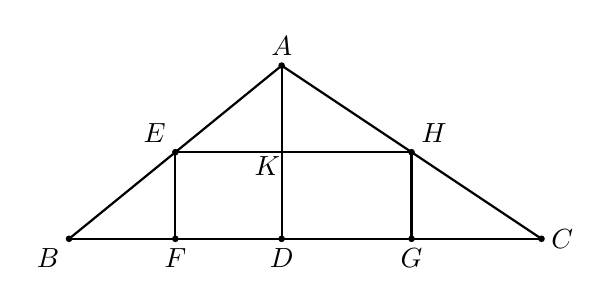
\begin{tikzpicture}[scale=1]
  \coordinate (B) at (0,0);
  \coordinate (C) at (6,0);
  \coordinate (A) at (2.7,2.2);
  \coordinate (D) at (2.7,0);
  \coordinate (E) at (1.35,1.1);
  \coordinate (H) at (4.35,1.1);
  \coordinate (F) at (1.35,0);
  \coordinate (G) at (4.35,0);
  \coordinate (K) at (2.7,1.1);
  \draw[thick] (B)--(C);
  \draw[thick] (A)--(B);
  \draw[thick] (A)--(C);
  \draw[thick] (A)--(D);
  \draw[thick] (E)--(H);
  \draw[thick] (E)--(F);
  \draw[thick] (H)--(G);
  \fill (A) circle (1.2pt) node[above] {$A$};
  \fill (B) circle (1.2pt) node[below left] {$B$};
  \fill (C) circle (1.2pt) node[right] {$C$};
  \fill (D) circle (1.2pt) node[below] {$D$};
  \fill (E) circle (1.2pt) node[above left] {$E$};
  \fill (F) circle (1.2pt) node[below] {$F$};
  \fill (G) circle (1.2pt) node[below] {$G$};
  \fill (H) circle (1.2pt) node[above right] {$H$};
  \node at (2.52,0.92) {$K$};
\end{tikzpicture}
